\chapter{Nonparametric Density Estimation}
This chapter is under \work.
\section{Histogram}
Let $x_1,\ldots,x_n$ be independent and identically distributed samples from a univariate continuous RV $X$ with density $f$. The simplest nonparametric estimator for $f$ is the histogram.  It has some serious drawbacks.  We have encountered the histogram earlier in \ref{S:ExploringData}.  During that encounter we chose the number of bins in an {\em ad hoc} fashion, often resorting to the default number of bins of $10$ in {\sc Matlab}'s {\tt hist} function.

A bin width that is too small when the number of bins is too large will give a histogram with many empty bins and many bins containing only a single data point.  This is referred as {\em under-smoothing}.  At the other extreme, a bin width that is too large due to a small number of bins results in a histogram that lacks details and results in {\em over-smoothing}.  In both of these situations, the histograms do not represent the underlying density well.

\begin{definition}[Density Histogram]
Let $x_1,\ldots,x_n$ be a random univariate sample with density $f$ and let $S_f$ be the support of $f$. Let $S_x\subset S_f$ be a connected interval containing $x_1,\ldots,x_n$ and let $\{B_1,\ldots,B_m\}$ be a finite contiguous partition of $S_x$ into $m$ bins of equal width $b$. For $x\in S_x$ and $B\in \{B_1,\ldots,B_m\}$, let $B(x)$ denote the bin that contains $x$. The {\it density histogram} for $x_1,\ldots,x_n$ with {\it bin width} $b$ is:
\begin{equation}
\widehat{f}_n(x,b)=\frac{1}{nb}\sum^n_{i=1}I_{B(x)}(x_i).
\end{equation}
\end{definition}

Hence, the density at $x$ is estimated by counting the number of sample points in the bin containing $x$, and then appropriately normalising this number so that the area covered by the histogram is 1.

%Consider the $a$-parametric family of the stretched oscillating exponential density with $\lambda = 9/20$, $\epsilon=1/2$:
%\[
%f_a(x) = a^{ {\lambda}^{-1} }{\Gamma (1+ {\lambda}^{-1})} \, \exp \{- a x^{\lambda} \}
%\left( 1 + \epsilon \, \sin ( a \, x^{\lambda} \, \tan( \lambda \pi  ) ) \right)
%\]

Now, let us consider the problem of estimating a histogram from $1500$ samples simulated from the equi-weighted mixture of $\normal(0,5^2)$, $\normal(10,1)$ and $\normal(-10,1)$ using the following code:
\begin{VrbM}
rand('twister',6898962)
randn('state',23121);
A=ceil(3*rand(1,2000));% Mixture Label vector
MuSs=[0 5; 10 2; -10 2]%; 5 2; -5 2]
x=arrayfun(@(i)(MuSs(i,1)+MuSs(i,2)*randn),A);
xgrid=-20:1:20;
pdf=NormalPdf(xgrid,MuSs(1,1),(MuSs(1,2))^2)/3 + NormalPdf(xgrid,MuSs(2,1),(MuSs(2,2))^2)/3 ...
    + NormalPdf(xgrid,MuSs(3,1),(MuSs(3,2))^2)/3;
\end{VrbM}

\begin{figure}[htpb]
\caption{Histogram estimates for the  with nine different bin-widths of $\{2,4,6,8,11,14,17,20,35\}$.  The fifth histogram with a bin-width of $11$ is the optimal one with the right amount of smoothing.  The ones with smaller bin-widths are under-smoothed and those with larger bin-widths are over-smoothed.\label{F:Gauss3MixHistsCV}}
\centering   \makebox{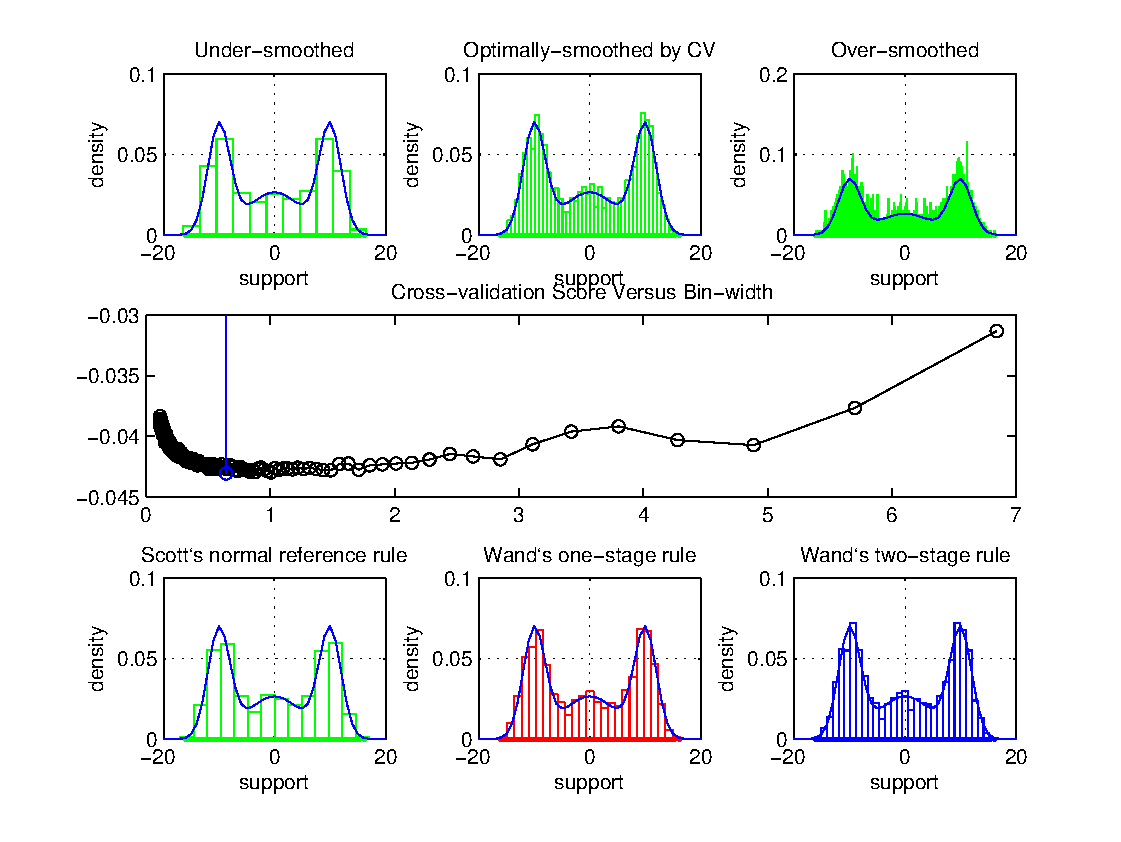
\includegraphics[width=6.5in]{figures/Gauss3MixHistsCV}}
\end{figure}

\subsubsection{Drawbacks of the histogram}
\begin{asparaenum}[(a)]
\item While densities of continuous random variables are continuous, the histogram is a step function with discontinuities.

\item The histogram does not use data efficiently\footnote{With an optimally chosen bin width, the mean integrated squared error, $E[\int [\widehat{f}_n(x,b)-f(x)]^2dx]$, converges to 0 at a rate of $n^{-2/3}$.}.

\item Although only one parameter, the bin width, appears explicitly in the definition of the histogram, the use of the histogram requires the specification of a second parameter. This is the placement of the leftmost bin edge, which can strongly affect the resulting histogram.
\end{asparaenum}

Because of these drawbacks, the histogram should only be used as a graphical tool for exploratory data analysis.


\subsubsection{Selection of histogram bin width}
\begin{asparaenum}[(a)]
\item	{\it Sturges' rule}: The number of bins is given by:
\begin{equation}
m=ceil(1+\log_2n).
\end{equation}
In practice, the bin width is usually obtained by:
\begin{equation}
b=\frac{x_{(n)}-x_{(l)}}{m}.
\end{equation}
\item	{\it Scott's normal reference rule}:
\begin{equation}
b=3.5\widehat{\sigma}n_{-1/3},
\end{equation}

where $\widehat{\sigma}$ is the sample standard deviation.

\item	{\it Freedman-Diaconis' rule}:
\begin{equation}
b=2(\widehat{q}_{0.75}-\widehat{q}_{0.25})n^{-1/3},
\end{equation}
where $\widehat{q}_p$ is the sample $p$-quantile.\\
With Scott's bin width or Freedman-Diaconis' bin width, the number of bins can be obtained by:
\begin{equation}
m= \lceil \left(\frac{x_{(n)}-x_{(1)}}{b}\right) \rceil.
\end{equation}
\end{asparaenum}

In practice, these methods for determining bin width should be used as starting points for trying several possible bin widths, with the final bin width chosen by visual inspection of the resulting histograms.

A suggestion for the placement of the leftmost bin edge is to use a {\em centred histogram}. For a histogram with $m$ bins and bin width $b$, $mb\geq x_{(n)}-x_{(1)}$, and so let:
\begin{equation}
\delta=mb-(x_{(n)}-x_{(1)}).
\end{equation}

To get the centred histogram, place the leftmost bin edge at $x_{(1)}-\delta/2$, so that the histogram extends equally by $\delta/2$ beyond the smallest and largest data values.
\subsubsection{{\sc Matlab} function for density histogram}

\VrbMf[label=histogram.m]{scripts/histogram.m}
%\begin{VrbM}
%% histogram.m
%% Plots density histogram for data in X.
%%
%% Usage: histogram(X, plot data, bounds, colour, bwmethod, bw);
%%
%% Input: X = row vector of data,
%%        plotdata (binary) = plot data points?
%%        bounds = [lower bound , upper bound] for possible X values,
%%        colour (single-character string) = colour of histogram (default =
%%        'y' for yellow),
%%        bwmethod (optional, default = 2) = method of computing bin width:
%%                 0 = Scott's normal reference rule,
%%                 1 = Wand's one-stage rule,
%%                 2 = Wand's two-stage rule,
%%                 3 = manual,
%%        bw = manual bin width if bwmethod = 3.
%%
%% Remark: Bin origin determined by centring the histogram, i.e. so that
%% left and right bin edges extend beyond min(X) and max(X) respectively
%% by equal amounts.
%%
%% Reference: Wand M.P. (1997), "Data-based choice of histogram bin width",
%% American Statistician 51, 59-64.
%\end{VrbM}

%\begin{example}[Shuttle Data] Joint temperatures of the O-rings for each test firing or actual launch of the space shuttle rocket motor are shown in the table below (from {\it Presidential Commission on the Space Shuttle Challenger Accident}).
%\begin{center}
%\begin{tabular}{|cccccccccc|}\hline
%\multicolumn{10}{|c|}{ O-ring temperatures ($^o$F)}\\\hline
%31   &  40&     45   &  49&     52   &  53&     57  &   58&     58  &   60\\
%61   &  61 &    63  &   66 &    67  &   67 &    67 &    67 &    68 &    69\\
%70    & 70  &   70 &    70  &   72 &    73  &   75&     75  &   76&     76\\
%78     &79   &  80&     81   &  83&     84&&&&\\\hline
%\end{tabular}
%\end{center}
%%\includegraphics
%\end{example}

%%% Dominic's material here
%\chapter{Density estimation}
%%\section{Histogram}
%WORK - fuse with previous material
Let $x_1,\ldots,x_n$ be a random univariate sample from a continuous distribution with density $f$. The most common nonparametric estimator for $f$ is the histogram, which has some serious drawbacks.
\subsection{\define}Let $x_1,\ldots,x_n$ be a random univariate sample with density $f$ and let $S_f$ be the support of $f$. Let $S_x\subset S_f$ be a connected interval containing $x_1,\ldots,x_n$ and let $\{B_1,\ldots,B_m\}$ be a finite contiguous partition of $S_x$ into $m$ bins of equal width $b$. For $x\in S_x$ and $B\in \{B_1,\ldots,B_m\}$, let $B(x)$ denote the bin that contains $x$. The {\it density histogram} for $x_1,\ldots,x_n$ with {\it bin width} $b$ is:
\begin{equation}
\hat{f}_H(x,b)=\frac{1}{nb}\sum^n_{i=1}I_{B(x)}(x_i).
\end{equation}
%\begin{flushright}   $\boxbox$ \end{flushright}

Hence, the density at $x$ is estimated by counting the number of sample points in the bin containing $x$, and then appropriately normalising this number so that the area of the histogram equals 1.

\begin{example}
Suppose $x_1,\ldots,x_{500}$ is a random sample drawn from the standard normal distribution. A histogram for $x_1,\ldots,x_{500}$ is shown in the figure:
%\includegraphics
%\begin{flushright}   $\boxbox$ \end{flushright}
\end{example}

\subsection{Drawbacks of the histogram}
\begin{asparaenum}[(a)]
\item While densities of continuous random variables are continuous, the histogram is a step function with discontinuities.

\item The histogram does not use data efficiently\footnote{With an optimally chosen bin width, the mean integrated squared error, $E[\int [\hat{f}_H(x,b)-f(x)]^2dx]$, converges to 0 at a rate of $n^{-2/3}$.}.

\item Although only one parameter, the bin width, appears explicitly in the definition of the histogram, the use of the histogram requires the specification of a second parameter. This is the placement of the leftmost bin edge, which can strongly affect the resulting histogram.
\end{asparaenum}
Because of these drawbacks, the histogram should only be used as a graphical tool for exploratory analysis.
%\begin{flushright}   $\boxbox$ \end{flushright}

\subsection{Selection of histogram bin width}
\begin{asparaenum}[(a)]
\item	{\it Sturges' rule}: The number of bins is given by:
\begin{equation}
m=ceil(1+\log_2n).
\end{equation}
In practice, the bin width is usually obtained by:
\begin{equation}
b=\frac{x_{(n)}-x_{(l)}}{m}.
\end{equation}
\item	{\it Scott's normal reference rule}:
\begin{equation}
b=3.5\hat{\sigma}n^{-1/3},
\end{equation}

where $\hat{\sigma}$ is the sample standard deviation.

\item	{\it Freedman-Diaconis' rule}:
\begin{equation}
b=2(\hat{q}_{0.75}-\hat{q}_{0.25})n^{-1/3},
\end{equation}
where $\hat{q}_p$ is the sample $p$-quantile.\\
With Scott's bin width or Freedman-Diaconis' bin width, the number of bins can be obtained by:
\begin{equation}
m=ceil\left(\frac{x_{(n)}-x_{(l)}}{b}\right).
\end{equation}
\end{asparaenum}
%\begin{flushright}   $\boxbox$ \end{flushright}

In practice, these methods for determining bin width should be used as starting points for trying several possible bin widths, with the final bin width chosen by visual inspection of the resulting histograms. A bin width that is too small will give a histogram with many empty bins and many bins containing only a single data point. At the other extreme, a bin width that is too large results in a histogram that lacks details. In both of these situations, the histograms do not represent the underlying density well.

\begin{example}[Shuttle data]
Joint temperatures of the O-rings for each test firing or actual launch of the space shuttle rocket motor are shown in the table below (from {\it Presidential Commission on the Space Shuttle Challenger Accident}).
\begin{center}
\begin{tabular}{|cccccccccc|}\hline
\multicolumn{10}{|c|}{ O-ring temperatures ($^o$F)}\\\hline
31   &  40&     45   &  49&     52   &  53&     57  &   58&     58  &   60\\
61   &  61 &    63  &   66 &    67  &   67 &    67 &    67 &    68 &    69\\
70    & 70  &   70 &    70  &   72 &    73  &   75&     75  &   76&     76\\
78     &79   &  80&     81   &  83&     84&&&&\\\hline
\end{tabular}
\end{center}
%\includegraphics
%\begin{flushright}   $\boxbox$ \end{flushright}
\end{example}

A suggestion for the placement of the leftmost bin edge is to use a \textquotedblleft centred histogram". For a histogram with $m$ bins and bin width $b$, $mb\geq x_{(n)}-x_{(l)}$, and so let:
\begin{equation}
\delta=mb-(x_{(n)}-x_{(l)}).
\end{equation}

To get the centred histogram, place the leftmost bin edge at $x_{(l)}-\delta/2$, so that the histogram extends equally by $\delta/2$ beyond the smallest and largest data values.
%\subsection{\Matlab {\it function for density histogram.}}
%\begin{VrbM}
%% histogram.m
%% Plots density histogram for data in X.
%%
%% Usage: histogram(X, plot data, bounds, colour, bwmethod, bw);
%%
%% Input: X = row vector of data,
%%        plotdata (binary) = plot data points?
%%        bounds = [lower bound , upper bound] for possible X values,
%%        colour (single-character string) = colour of histogram (default =
%%        'y' for yellow),
%%        bwmethod (optional, default = 2) = method of computing bin width:
%%                 0 = Scott's normal reference rule,
%%                 1 = Wand's one-stage rule,
%%                 2 = Wand's two-stage rule,
%%                 3 = manual,
%%        bw = manual bin width if bwmethod = 3.
%%
%% Remark: Bin origin determined by centring the histogram, i.e. so that
%% left and right bin edges extend beyond min(X) and max(X) respectively
%% by equal amounts.
%%
%% Reference: Wand M.P. (1997), "Data-based choice of histogram bin width",
%% American Statistician 51, 59-64.
%\end{VrbM}

\section{Kernel density estimation}
The {\it kernel density estimator} is a nonparametric estimator for $f$ that is continuous, uses data more efficiently than the histogram, and has only one parameter.

\begin{definition}
Let $x_1,\ldots,x_n$ be a random univariate sample with density $f$, and let $K$ be a function satisfying:
\begin{equation}
\int K(x)dx=1.
\end{equation}

The {\it kernel density estimator} for $f$ with bandwidth $h > 0$ and kernel $K$ is:
\begin{equation}
\hat{f}_K(x,h)=\frac{1}{nh}\sum^n_{i=1}K\left(\frac{x-x_i}{h}\right).
\end{equation}

We shall consider kernel functions that are densities and define:
\begin{equation}
K_h(x)=\frac{1}{h}K\left(\frac{x}{h}\right),
\end{equation}
and so the kernel density estimator can be expressed as:
\begin{equation}
\hat{f}_K(x,h)=\frac{1}{n}\sum^n_{i=1}K_h(x-x_i),
\end{equation}
which is a proper density.
\end{definition}

%\begin{flushright}   $\boxbox$ \end{flushright}
\subsection{Examples of kernel functions}

\begin{table}[tbh]
\centering
$$\begin{array}{|c|c|c|c|}\hline
\textrm{Name}&	K(x)	&\textrm{Efficiency}&\sigma_K\\
Epanechnikov	&\frac{3}{4}(1-x^2)I_{[-1,1]}(x)&1&\frac{1}{\sqrt{5}}	 \\
Biweight	 &\frac{15}{16}(1-x^2)^2I_{[-1,1]}(x)&0.994	 &\frac{1}{\sqrt{7}}\\
Triweight	 &\frac{35}{32}(1-x^2)^3I_{[-1,1]}(x)&0.987	 &\frac{1}{3}\\
Triangle&(1-|x|)I_{[-1,1]}(x)&0.986	 &\frac{1}{\sqrt{6}}\\
Gaussian&\frac{1}{\sqrt{2\pi}}\exp\left(-\frac{x^2}{2}\right)	 &0.951&	1\\
Uniform&\frac{1}{2}I_{[-1,1]}(x)&0.930&\frac{1}{\sqrt{3}}	 \\\hline
\end{array}$$
\end{table}
%\includegraphics
%\begin{flushright}   $\boxbox$ \end{flushright}
It turns out that the choice of the kernel has little impact on the performance of the kernel density estimator, and so the convenient Gaussian kernel is a popular choice. The choice of bandwidth, on the other hand, is critical.

\begin{prop}
Let $\sigma^2_K$ be the variance of kernel function $K$. The variance of $K_h(x)$ is $h^2\sigma^2_K$.

\begin{proof}
Since $K_h(x)$ has mean 0, its variance is:
$$ \sigma_K^2=\int x^2K_h(x)dx=\frac{1}{h}\int x^2K(x/h)dx=h^2\int (x/h)^2K(x/h)d(x/h)=h^2\sigma^2_K.$$
%\begin{flushright}   $\boxbox$ \end{flushright}
\end{proof}
\end{prop}

Note that for the Gaussian kernel, $\sigma_K=1$, and therefore $\sigma_K=h$; i.e. the standard deviation of $K_h$ is equal to its bandwidth.

\begin{labwork}
Using the same standard normal sample from Example 5.1.2, the density estimate obtained from a Gaussian kernel density estimator (with bandwidth 0.3) is shown in the figure, along with the histogram obtained previously.
%\includegraphics
%\Matlab code:
\begin{VrbM}
n = 500;
x = randn(1,n);
bw = 0.3;
s = [-3:0.01:3]; % support points to compute density
f = normpdf(s,0,1); % true N(0,1) density
ns = length(s); % number of support points
fker = zeros(1,ns); % storage for kernel density
for i = 1:ns
    fker(i) = mean(normpdf(s(i),x,bw));
end
histogram(x,0,[-inf inf],'g'); hold on
plot(s,f,':r',s,fker,'-r')
\end{VrbM}
%\begin{flushright}   $\boxbox$ \end{flushright}
\end{labwork}

We can think of the kernel as spreading a probability mass of $1/n$ associated with each sample point around its neighbourhood. To see what the Gaussian kernel density estimator does, suppose we have only five sample points, $x_1,\ldots,x_5$. The estimator puts a normal density with variance $h^2$ and a probability mass of $1/n$ at each sample point, and estimates the density at support point $x$ by summing the contributions from these normal densities at $x$. This is illustrated in the figure, where the sample points are marked by \textquoteleft x' on the support axis, the dashed curves are the normal densities whose probability masses are scaled to $1/n$, and the solid curve is the estimated density.
%\includegraphics

If f is continuous at $x$ and $h\rightarrow 0$ and $nh\rightarrow\infty$ as $n\rightarrow\infty$, then for any $\epsilon > 0$:
\begin{equation}
\lim_{n\rightarrow\infty}P(|\hat{f}_K(x,h)-f(x)|\leq\epsilon)=1.
\end{equation}
%\begin{flushright}   $\boxbox$ \end{flushright}

\subsection{Bandwidth selection}
The use of the kernel density estimator requires the specification of the bandwidth, which plays a similar role as the histogram's bin width. A practical and easy-to-use bandwidth choice for the Gaussian kernel is {\it Scott's bandwidth}:
\begin{equation}
h=\hat{s}n^{-1/5},
\end{equation}

where $\hat{s}=\min\{\hat{\sigma},(\hat{q}_{0.75}-\hat{q}_{0.25})/1.348\}$. A slightly different version\footnote{This version is also known as the {\it normal reference rule.}} of Scott's bandwidth is given by:
\begin{equation}
h=1.06\hat{s}n^{-1/5}.
\end{equation}

Since the multiplicative constant of 1.06 is very close to 1, the two bandwidths are very close and we can use either of them.

A more sophisticated bandwidth can be obtained by considering the minimisation of {\it asymptotic mean integrated squared error}:
\begin{equation}
AMISE=\lim_{n\rightarrow\infty}E[\int[\hat{f}_K(x,h)-f(x)]^2dx].
\end{equation}

Using $R(g)$ to denote $\int g(x)^2dx$, the resulting optimal bandwidth is given by:
\begin{equation}
h_{AMISE}=\left(\frac{R(K)}{n\sigma^4_KR(f^{\prime\prime})}\right)^{1/5},
\end{equation}

which depends on the unknown density $f$ through $R(f^{\prime\prime})$. An approximate bandwidth is obtained by plugging in an appropriate estimate of $R(f^{\prime\prime})$\footnote{Sheather, S. J. and Jones, M. C. (1991), \textquotedblleft A reliable data-based bandwidth selection method for kernel density estimation", {\it Journal of the Royal Statistical Society, Series B, 53, 683-690}.}.

With an optimally chosen bandwidth, the mean integrated squared error of the kernel density estimator converges to 0 at rate $n^{4/5}$.
%\begin{flushright}   $\boxbox$ \end{flushright}

%\subsection{\result}
Let $K$ and $L$ be two kernel functions with standard deviations $\sigma_K$ and $\sigma_L$ respectively. Then for the resulting kernel densities to be approximately equal, their bandwidths, $h_K$ and $h_L$, must satisfy:
\begin{equation}
h_K\sigma_K\approx h_L\sigma_L,
\end{equation}
i.e. the standard deviations of $K_h$ and $L_h$ must be approximately equal.
%\begin{flushright}   $\boxbox$ \end{flushright}

Recall that the standard deviation of the Gaussian kernel function is 1, so we can use this result to obtain the bandwidth for some other kernel, e.g. kernel function $K$, from the bandwidth of the Gaussian kernel:
\begin{equation}
h_K\approx \frac{h_{gaussian}}{\sigma_K}.
\end{equation}

For example, with the Epanechnikov kernel, $\sigma_K=1/\sqrt{5}$, and so Scott's bandwidth for the Epanechnikov kernel is:$$h_K\approx\sqrt{5}\hat{s}n^{-1/5}.$$

\begin{labwork}
The data in {\tt geyser.txt} are 107 durations (in minutes) of the eruptions of the Old Faithful geyser. Compare the kernel density estimates for eruption duration using the Gaussian and Epanechnikov kernels with Scott's bandwidth.

%\Matlab code:
\begin{VrbM}
x = load('geyser.txt');
n = length(x);
n5 = n^(-0.2);
hscottgauss = min(std(x),iqr(x)/1.348) * n5 % Scott's bandwidth for Gaussian
			% kernel
hscottepan = sqrt(5) * hscottgauss % Scott's bandwidth for Epanechnikov kernel
\end{VrbM}
Results:
\begin{VrbM}
hscottgauss = 0.4087
hscottepan = 0.9139
\end{VrbM}
%\includegraphics
%\caption{Kernel densities with Scott's bandwidth (solid curve) and optimal bandwidth (dashed curve).}
%\begin{flushright}   $\boxbox$ \end{flushright}
\end{labwork}

\subsection{Adjustment at boundaries}
Suppose we need to estimate a density $f$ whose support $S_f$ is bounded at one or both ends; frequently, $S_f=(0,\infty)$ or $S_f=(a,b)$. The presence of a boundary or boundaries may cause some of the kernels in the kernel density estimator to be truncated. Therefore, the estimator must be adjusted accordingly to ensure that the resulting estimate remains a density:
\begin{equation}
\hat{f}_K(x,h)=\frac{1}{n}\sum^n_{i=1}\frac{K_h(x-x_i)}{p_i},
\end{equation}
where:
\begin{equation}
p_i=\int_SK_h(x-x_i)dx.
\end{equation}

Thus, $0<p_i\leq 1$, and $p_i  = 1$ if the corresponding kernel is not truncated.

If the Gaussian kernel is used and letting $\Phi(t;\mu,\sigma^2)$ denote the cumulative probability at $t$ of the normal distribution with mean $\mu$ and variance $\sigma^2$, then:
\begin{equation}
p_i=1-\Phi(0;x_i,h^2),
\end{equation}
when $S_f=(0,\infty)$, and:
\begin{equation}
p_i=\Phi(b;x_i,h^2)-\Phi(a;x_i,h^2),
\end{equation}
when $S_f=(a,b)$.
%\begin{flushright}   $\boxbox$ \end{flushright}

\begin{labwork}
Let $x_1,\ldots,x_{100}$ be a sample from an exponential distribution with parameter 1. Recall the the support of the exponential distribution is $x \geq 0$.
%\includegraphics
%\Matlab code:
\begin{VrbM}
n = 100;
x = exprnd(1,1,n); % n exponential(1) random variables
n5 = n^(-0.2);
h = min(std(x),iqr(x)/1.348) * n5; % Scott's bandwidth for Gaussian kernel
s = [0:0.01:4]; % support points to compute density
f = exppdf(s,1); % true exponential(1) density
ns = length(s); % number of support points
fker1 = zeros(1,ns); % storage for kernel density without boundary correction
fker2 = zeros(1,ns); % storage for kernel density with boundary correction
p = 1 - normcdf(0,x,h); % boundary correction factors
for i = 1:ns
    fker1(i) = mean(normpdf(s(i),x,h)); % kernel density without boundary
		% correction
    fker2(i) = mean(normpdf(s(i),x,h)./p); % kernel density with boundary
		% correction
end
plot(s,f,'-b',s,fker2,'--b',s,fker1,':b')
legend('true density','kernel density with correction','kernel density without correction')
\end{VrbM}
%\begin{flushright}   $\boxbox$ \end{flushright}
\end{labwork}

\section{Extension to multivariate data}
The extension of the kernel density estimator to multivariate data is straightforward.

%\begin{definition}
Let $x_1,\ldots,x_n$ be independent and identically distributed random $d$-vectors with $d$-dimensional density $f$. The kernel density estimator for $f$ is:
\begin{equation}
\hat{f}_K(x,H)=\frac{1}{n|H|}\sum^n_{i=1}K(H^{-1}(x-x_i)),
\end{equation}
where $H$ is a $d \times d$ nonsingular matrix, called the {\it bandwidth matrix}, and the kernel function $K$ is a $d$-dimensional density. Let:
\begin{equation}
K_H(x)=\frac{K(H^{-1}x)}{|H|},
\end{equation}

so that:
\begin{equation}
\hat{f}_K(x,H)=\frac{1}{n}\sum^n_{i=1}K_H(x-x_i).
\end{equation}

The kernel can be simplified by assuming that its components are independent (note that this does not make the components of $x$ independent). This simplifies the kernel matrix to a diagonal matrix with diagonal elements, $h_1,\ldots,h_d$. The kernel can then be expressed as a product of univariate kernels:
\begin{equation}
K_H(x)=K_{h_1,\ldots,h_d}(x)=\prod^d_{j=1}K_{h_j}[x(j)],
\end{equation}
where $x(j)$ denotes the $j^{\textrm{th}}$ component of $x$. This gives the {\it product kernel density estimator}:
\begin{equation}
\hat{f}_K(x,h_1,\ldots,h_d)=\frac{1}{n}\sum^n_{j=1}[\prod^d_{j=1}K_{h_j}[x(j)-x_i(j)]].
\end{equation}
%\begin{flushright}   $\boxbox$ \end{flushright}
%\end{definition}

\subsection{Bandwidth selection}
For a product kernel density estimator with the Gaussian kernel, {\it Scott's rule in d dimensions} is:
\begin{equation}
h_j=\hat{s}_jn^{-1/4+d},
\end{equation}
where $\hat{s}_j=\min(\hat{\sigma}_j,(\hat{q}_{0.75j}-\hat{q}_{0.25j})/1.348)$ is the estimate of scale for the $j^{\textrm{th}}$ component that has been computed from $x_1(j),\ldots,x_n(j)$. For some other kernel, the required bandwidth may be obtained by dividing $h_j$ by the standard deviation of that kernel function, as in the univariate case.

With an optimally chosen bandwidth, the mean integrated squared error of the multivariate kernel density estimator converges to 0 at rate $n^{-4/(4+d)}$. Thus, its efficiency decreases rapidly with increasing dimension.
%\begin{flushright}   $\boxbox$ \end{flushright}

\begin{labwork}
The file {\tt nrl.txt} contains data from 42 rugby league matches.  The first column contains the length of game time, in seconds, until the first points are scored by a kick between the posts (penalty, drop goal or conversion); the second column contains the game time (in seconds) until the first try is scored. Denoting the log of the bivariate sample points by $(x_1,y_1),\ldots,(x_42,y_42)$, the product Gaussian kernel density estimator for the bivariate density is:
$$\hat{f}_\phi(x,y,h_x,h_y)=\frac{1}{42}\sum^{42}_{i=1}\phi(x,x_i,h^2_x)\phi(y,y_i,h_y^2).$$

Using Scott's rule:
$$h_x=\hat{s}_x\times 42^{-1/6} \textrm{  and   }h_y=\hat{s}_y\times 42^{-1/6}.$$
%\includegraphics
%\Matlab code:
\begin{VrbM}
data = load('nrl.txt');
x = log(data(:,1))';
y = log(data(:,2))';
n = length(x);

% scatter plot:
plot(x,y,'.r')
xlabel('x'), ylabel('y')
title('Scatter plot')
axis([3 9 3 9]), axis('square')
drawnow

n6 = n^(-1/6);
hx = min(std(x),iqr(x)/1.348) * n6;
hy = min(std(y),iqr(y)/1.348) * n6;
s = 3:.01:9;
ns = length(s);
phix = zeros(n,ns);
phiy = zeros(n,ns);
for i = 1:n
    phix(i,:) = normpdf(s,x(i),hx);
    phiy(i,:) = normpdf(s,y(i),hy);
end
fker = zeros(ns,ns);
for j = 1:ns
    for i = 1:ns
        fker(j,i) = phiy(:,j)' * phix(:,i) / n;
    end
end

% 3-D surface plot:
figure, mesh(s,s,fker)
xlabel('x'), ylabel('y'), zlabel('density')
colorbar, drawnow

% contour plot:
figure, contourf(s,s,fker,20)
xlabel('x'), ylabel('y')
title('Contour plot')
colorbar, axis('square')
\end{VrbM}
%\begin{flushright}   $\boxbox$ \end{flushright}
\end{labwork}

\section{Smoothed bootstrap}
The {\it smoothed bootstrap} is a variation of the bootstrap idea that is used for continuous data. Instead of estimating the distribution function by the EDF and obtaining bootstrap samples by random sampling with replacement from the data values, the smoothed bootstrap estimates the density by a kernel density and generates bootstrap samples from it. After getting the bootstrap samples, the MSE, variance, bias and confidence intervals can be computed for an estimator of interest, in the same way as in the nonparametric bootstrap. If the kernel density is a good estimate of the data density, then the smoothed bootstrap can give a small improvement over the nonparametric bootstrap for continuous data.

\subsection{Generating from a kernel density}
Let:$$\hat{f}_K(x,h)=\frac{1}{n}\sum^{n}_{i=1}K_h(x-x_i),$$
 be the kernel density.  To generate a new sample point from the kernel density, randomly pick one of the original data values, $x_1,\ldots,x_n$. Suppose   is picked, generate the new sample point from the kernel centred on $x_i$, i.e. from $K_h(x-x_i)$.
%\begin{flushright}   $\boxbox$ \end{flushright}

\begin{labwork}
Generate 1000 random values from the Gaussian kernel density, with Scott's bandwidth, for the geyser data.
%\Matlab code:
\begin{VrbM}
m = 1000; % number of sample points to generate
x = load('geyser.txt')';
n = length(x);
n5 = n^(-0.2);
h = min(std(x),iqr(x)/1.348) * n5; % Scott's bandwidth for Gaussian kernel
xcen = randsample(x,m,true); % randomly resample kernel centres from x
y = normrnd(xcen,h); % generate from Gaussian kernels centred at xcen
histogram(y,0,[0 inf],'r');
\end{VrbM}
%\includegraphics
%\begin{flushright}   $\boxbox$ \end{flushright}
\end{labwork}

\subsection{Smoothed bootstrap procedure for generating bootstrap samples}
Let $x_1,\ldots,x_n$ be IID random variables with unknown density $f(x)$.
\begin{asparaenum}[(a)]
\item Estimate the data density by a kernel density $\hat{f}_K(x,h)$.

\item	Obtain $N$ bootstrap samples, each of size $n$, by generating from $\hat{f}_K(x,h)$:
$$\begin{array}{c}
\{x_{1,1},\ldots,x_{1,n}\}\sim\hat{f}_K(x,h)\\
\textrm{M}\\
\{x_{N,1},\ldots,x_{N,n}\}\sim\hat{f}_K(x,h)\\
\end{array}$$
\end{asparaenum}
%\begin{flushright}   $\boxbox$ \end{flushright}

\begin{labwork}
Let us revisit Example 4.2.5 to obtain a 0.95 percentile interval for the median amount of sodium using the smoothed bootstrap with a Gaussian kernel density. Recall that the percentile interval provided by the nonparametric bootstrap was $(75.05, 77)$.

%\Matlab code:
\begin{VrbM}
x = load('sodium.txt'); % load data from text file and store in x
N = 100000; % number of bootstrap samples
n = length(x); % determine number of data values
nN = n * N;
alpha = 0.05;
alpha2 = alpha / 2;
alpha21 = 1 - alpha2;
n5 = n^(-0.2);
h = min(std(x),iqr(x)/1.348) * n5; % Scott's bandwidth for Gaussian kernel
xcen = randsample(x,nN,true); % randomly resample kernel centres from x
xboot = normrnd(xcen,h); % generate from Gaussian kernels centred at xcen
xboot = reshape(xboot,n,N); % organise resampled values into N columns of n
                            		% values each so that each column is a bootstrap
                            		% sample of size n
xbootmed = median(xboot); % medians of bootstrap samples
xbootmedsort = sort(xbootmed); % sort medians in increasing order

% (1-alpha) percentile interval:
[xbootmedsort(ceil(N*alpha2)) xbootmedsort(N*alpha21)]
\end{VrbM}
Results:
\begin{VrbM}
ans = 74.8616   76.9451
\end{VrbM}
Therefore, a 0.95 percentile interval for the median amount of sodium, using the smoothed bootstrap with a Gaussian kernel density, is $(74.86, 76.95)$.
%\begin{flushright}   $\boxbox$ \end{flushright}
\end{labwork}


Point-wise confidence band for density using the smoothed bootstrap (see Scott\footnote{Scott, D.W. (1992), {\it Multivariate Density Estimation: Theory, Practice and Visualization, Wiley.}} pp. 259-260; Hardle et al.\footnote{Hardle, W., Muller, M., Sperlich, S. and Werwatz, A. (2004), {\it Nonparametric and Semiparametric Models,} e-book at www.quantlet.com/mdstat/scripts/spm/html/spmhtmltoc.html}  section 3.5).

\section{Exercises}

\begin{exercise}
Consider the two-component normal mixture density given by:
$$f(x)=0.5\phi(x,4,1)+0.5\phi(x,9,4),$$

where $\phi(x,\mu,\sigma^2)$ denotes the normal density with mean $\mu$ and variance $\sigma$, evaluated at $x$.
\begin{asparaenum}[(a)]
\item A sample point, $x$, can be generated from the mixture density by the following algorithm:
\begin{tabbing}
Gene\=rate $u \sim U[0, 1]$.\\
If $u\leq 0.5$\\
	\>Generate $x \sim N(4, 1)$\\
Else\\
	\>Generate $x \sim N(9, 4)$.\\
\end{tabbing}

Implement a \Matlab function to generate from the mixture density and use it to get 100 sample points.

\item Using the 100 sample points from part (a), estimate the underlying density using a histogram with appropriate bin width. Explain clearly how you arrived at your choice of bin width.

\item Using the 100 sample points from part (a), estimate the underlying density using a Gaussian kernel density estimator. Explore bandwidths ranging from 0.3 to 1.9 to decide on an appropriate one.
\end{asparaenum}
\end{exercise}

\begin{exercise}
The Bart Simpson density is given by:
$$f(x)=0.5\phi(x,0,1)+0.1\sum^4_{j=0}\phi(x,0.5j-1,0.01).$$

To see why it is called the Bart Simpson density, plot the density for a sequence of x values from $-3$ to 3 (in steps of 0.01, for example).
\begin{asparaenum}[(a)]
\item Write a \Matlab function to generate sample points from the Bart Simpson density and use it to obtain 1000 sample points.
\item Using the 1000 sample points from part (a), estimate the underlying density using a histogram with appropriate bin width. Explain clearly how you arrived at your choice of bin width.
\item Using the 1000 sample points from part (a), estimate the underlying density using a Gaussian kernel density estimator with bandwidths of 0.005, 0.05 and 0.5. Comment on the performance of each of these bandwidths.
\end{asparaenum}
\end{exercise}

\begin{exercise}
The data in {\tt ceo.txt} contain the ages (column 1) and salaries (column 2, in thousands of dollars) of the CEOs of 59 companies.
\begin{asparaenum}[(a)]
\item Obtain a Gaussian kernel density estimate for the salaries, using Scott's bandwidth. Compare the transformation method and boundary correction method for handling the boundary at zero.

\item Use the nonparametric bootstrap to obtain a point-wise 0.95 BCA confidence band for the density of the salaries.

\end{asparaenum}
\end{exercise}

\begin{exercise}
The second column of {\tt glass.txt} contains measurements of the refractive index of 214 glass specimens collected in forensic work.
\begin{asparaenum}[(a)]
\item Obtain a Gaussian kernel density estimate for refractive index, using Scott's bandwidth.

\item Use the nonparametric bootstrap to obtain a point-wise 0.95 BCA confidence band for the density of refractive index.
\end{asparaenum}

\end{exercise}

\begin{exercise}
The data in {\tt whale.txt} are the times of 121 bowhead whale calf sightings during the 2001 spring migration. The time of each sighting is expressed as the number of hours since midnight of April 5, when the first adult whale was sighted.
\begin{asparaenum}[(a)]
\item Plot a density histogram for the data and superimpose onto it a Gaussian kernel density estimate. Explain your choice of histogram bin width and kernel density bandwidth. For the kernel density estimate, compare the transformation method and the boundary correction method for handling the boundary at zero.

\item Obtain a 0.95 BCA interval for the median sighting time, using the nonparametric bootstrap with 10,000 bootstrap samples.

\item Repeat Part (b) using the smoothed bootstrap with 10,000 bootstrap samples.
\end{asparaenum}

\end{exercise}

\begin{exercise}
The data in {\tt density.txt} are 29 measurements of the density of the earth, which were made by Henry Cavendish in 1789.
\begin{asparaenum}[(a)]
\item Plot a density histogram for the data and superimpose onto it a Gaussian kernel density estimate. Explain your choice of histogram bin width and kernel density bandwidth. For the kernel density estimate, compare the transformation method and the boundary correction method for handling the boundary at zero.
\item Obtain a 0.95 BCA interval for the mean density of the earth, using the nonparametric bootstrap with 10,000 bootstrap samples.
\item Repeat Part (b) using the smoothed bootstrap with 10000 bootstrap samples.
\end{asparaenum}

\end{exercise}

\begin{exercise}
Work through Example 5.3.3 for the NRL data.
\end{exercise}

\begin{exercise}
The data in {\tt infrared.txt} are measurements of infrared emissions from 628 objects beyond our galaxy. The two columns contain total flux measurements for two different wavelength bands - the first column shows the 12 micrometre band and the second column shows the 100 micrometre band. Estimate the bivariate density for the log of the data using a product Gaussian kernel density estimator with Scott's bandwidth. Plot the estimated density using a three-dimensional surface plot and a two-dimensional contour plot.
\end{exercise} 
